\documentclass[11pt]{article}
\usepackage[review]{acl}
\usepackage{times}
\usepackage{latexsym}
\usepackage[T1]{fontenc}
\usepackage[utf8]{inputenc}
\usepackage{microtype}
\usepackage{inconsolata}
\usepackage{graphicx}
\usepackage{amsmath,amssymb}
\usepackage{booktabs}
\usepackage{array}

% Working draft. Add empirical claims only after completing the experiments.
% Keep the official ACL style, font sizes, margins, and title box unchanged.
\title{Waterfall: Unified Agentic Search and Recommendation\\
through Continual User Modeling and Feedback}
\author{Anonymous ACL submission}

\begin{document}
\maketitle

\begin{abstract}
Personal information feeds must decide what to search for, which retrieved items to show, and what to learn from subsequent interaction. These decisions depend on the same evidence, yet a poor recommendation does not identify which decision failed. A request for easier tutorials may require a different query, a different ordering of existing candidates, or a revision to the user's inferred expertise. We formulate this problem as budgeted coordination of acquisition, ranking, and user-state updates over successive interactions. We describe Waterfall, a framework that translates language instructions and behavior into scoped state changes and uses the resulting state to coordinate these operations. An existing prototype supports bounded memory and query updates; we specify a broader controller that also conditions acquisition and reranking on the available candidates. We develop an evaluation protocol combining a published agent recommendation benchmark, a proposed multi-round extension, and real behavioral logs. The protocol separates recommendation usefulness, adaptation, and resource cost. This draft reports the formulation and method design; the broader controller and empirical evaluation remain to be completed.
\end{abstract}

\section{Introduction}
\label{sec:intro}

A user who has just bought a camera no longer needs a feed dominated by camera reviews. They may instead want short lessons on taking photographs. If the next lessons are too advanced, the system must decide what to change. It could search for introductory material, promote suitable lessons already in its candidate pool, or revise its estimate of the user's experience. These choices have different costs and different consequences for later recommendations.

The feedback itself rarely specifies the required operation. ``These are too advanced'' identifies a mismatch in difficulty, but does not imply a dislike of photography. ``I have already seen these'' concerns novelty, not necessarily preference. A short visit is less specific still: the item may be irrelevant, familiar, slow to load, or simply interrupted. Treating each observation as a new permanent interest can distort the profile. Responding to every observation with another search can spend resources without improving the feed.

Language agents offer a way to interpret such feedback and act across recommendation stages. Existing work already covers much of this space. InteRecAgent orchestrates recommendation tools \citep{huang2025interecagent}; RecBot interprets active user commands \citep{tang2026recbot}; MARS maintains hierarchical preference memory \citep{shen2026mars}. ClawRec connects user state, source planning, acquisition, slate construction, and feedback \citep{wu2026clawrec}. The presence of these components in one system is therefore insufficient to establish a new contribution.

We instead study \emph{how their updates should be coordinated}. A useful controller needs to distinguish a shortage of suitable candidates from a poor ordering of candidates that are already available. It must also decide whether new evidence applies to the current task or to a more persistent preference. These distinctions connect language interpretation to concrete downstream decisions: the same correction should affect both future queries and current ranking when appropriate, while leaving unrelated preferences intact.

Our research question is whether coordinating these decisions improves recommendations over successive interactions under a common resource budget. The comparison is against systems with the same information and tools, including a fixed pipeline with shared user state and a general tool-using agent. This framing tests whether a coordination mechanism adds value beyond giving each stage more context.

Waterfall provides a prototype from which to study this question. Its current code path allows an agent to propose bounded memory and search-term edits, while application logic retrieves and ranks content. We specify an extension in which the controller also inspects the candidate pool before choosing acquisition, reranking, or no change. Throughout this paper, \emph{adaptation} means updating runtime state and actions; the language model's parameters remain frozen.

The draft develops three parts of the study: a formulation of continual search and recommendation with explicit action boundaries; a coordination method connecting feedback scope to acquisition and ranking; and an evaluation design that measures effects across interactions rather than only on a final static list. The existing implementation and proposed extension are separated in Section~\ref{sec:prototype}. No quantitative result or improvement claim is made at this stage.

\section{Related Work}
\label{sec:related}

\paragraph{Agents for recommendation.}
InteRecAgent integrates retrieval and ranking tools through an LLM agent \citep{huang2025interecagent}. RecBot parses active commands and plans operations over recommendation candidates \citep{tang2026recbot}. These systems establish tool orchestration and command-driven recommendation as prior work. We include a ReAct-style controller \citep{yao2023react} with Waterfall's state and action interface to test whether general tool use is sufficient for the proposed task.

\paragraph{User memory and control.}
MARS organizes interaction evidence into preference chunks and a higher-level profile, with operations for updating and consolidating memory \citep{shen2026mars}. iAgent places an LLM agent between users and recommender systems to support user control \citep{xu-etal-2025-iagent}. These approaches motivate explicit memory operations. Our focus is their effect across stages: whether the scope of a state edit can coordinate acquisition and ranking without introducing unnecessary updates.

\paragraph{Complete workflows.}
ClawRec is the closest architectural comparison: it already connects evolving user state with source-aware acquisition, recommendation, and feedback \citep{wu2026clawrec}. Its main benchmark evaluates recommendations from a supplied history prefix with held-out behavior. This supplies a useful shared starting point, but repeated interaction with each method's own recommendations requires an additional protocol. Our proposed multi-round study targets that distinction in evaluation; it does not imply that ClawRec lacks a feedback mechanism.

\paragraph{Coupling retrieval and ranking.}
RRCM uses ranking feedback to learn retrieval over collaborative and metadata memories \citep{li2026rrcm}. Retrieval-augmented conversational recommendation also optimizes retrieval using recommendation rewards \citep{yue2026rar}. Thus, downstream ranking quality has already been used to guide retrieval. Our proposed setting adds persistent user-state edits and decisions about whether acquisition is needed at all, with frozen model parameters. Whether this distinction yields an effective method must be established against strong coupled systems.

\paragraph{Behavioral and textual data.}
KuaiRand provides sequential feedback, including explicit reactions and playback-related signals \citep{gao2022kuairand}. MIND provides news content and impression-level click data \citep{wu2020mind}. These resources can test parts of the feedback and ranking pipeline, but neither supplies the full counterfactual trajectory of a new multi-source agent. We therefore distinguish evaluation on recorded behavior from interaction generated in response to a tested policy.

\section{Task Formulation}
\label{sec:task}

We consider a user consuming a sequence of recommendation slates. At decision step $t$, the system observes a history $H_t$ containing only information available up to that step. An observation may be a language instruction, an explicit reaction, or an exposure event with source-dependent interaction metadata. The user's underlying goal is not directly observable.

The system maintains the state
\begin{equation}
z_t = (U_t,M_t,Q_t,C_t,H_t,b_t),
\end{equation}
where $U_t$ represents explicit requirements, $M_t$ inferred preferences, $Q_t$ acquisition queries, $C_t$ available candidates, and $b_t$ the remaining budget. Explicit instructions and inferred preferences remain distinguishable. Candidates carry source and availability information; an unsuccessful source request is not represented as negative user feedback.

The action interface contains four operations:\par\nopagebreak
\begin{itemize}
    \item \textsc{Edit}: revise an allowed portion of user state or the query plan;
    \item \textsc{Acquire}: request more candidates through authorized sources;
    \item \textsc{Rank}: select and order a slate from available candidates;
    \item \textsc{Hold}: retain the current state or ordering until further evidence arrives.
\end{itemize}
An interaction can require several operations. For example, a difficulty correction can produce a state edit followed by reranking, with acquisition needed only if the current pool lacks suitable material.

Let $L_t$ be the displayed slate and $y_t(x)\in\{0,1,2\}$ the evaluation judgment for item $x$: unsuitable, partially useful, or useful for the current goal. These labels are unavailable to the controller. We define a trajectory objective
\begin{equation}
\max_{\pi}\ \mathbb{E}_{\pi}
\left[\sum_{t=1}^{T}\sum_{x\in L_t}
\nu_t(x)\,\mathbf{1}\{y_t(x)=2\}\right],
\label{eq:objective}
\end{equation}
subject to resource limits. Here $\nu_t(x)=1$ only on the first exposure to the item's duplicate group in the trajectory. The policy $\pi$ therefore receives no additional utility for repeatedly showing the same useful content. The budget has separate limits for model tokens and source calls; latency is reported alongside quality. Equation~\ref{eq:objective} defines the evaluation target, not an objective that the current prototype has been trained to optimize.

\section{Coordinated Control in Waterfall}
\label{sec:method}

This section specifies the proposed full controller. It extends the prototype's bounded edits with candidate-aware action selection. Figure~\ref{fig:loop} shows the intended information flow. Neither the extension nor its effectiveness is claimed as an implemented result.

\begin{figure*}[t]
\centering
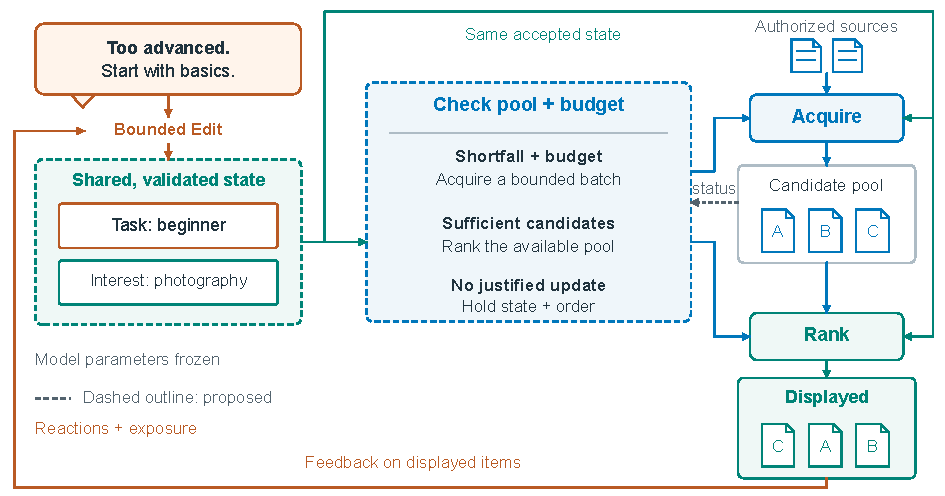
\includegraphics[width=\textwidth]{figures/waterfall-architecture.pdf}
\caption{Proposed Waterfall controller. A difficulty correction updates task state while retaining a persistent photography interest. The policy edits shared state and inspects candidate sufficiency and budget before acquiring content, reranking available items, or holding. Letters denote illustrative item identifiers. Dashed modules are proposed extensions; solid modules are existing component types.}
\label{fig:loop}
\end{figure*}

\subsection{Preserving the Meaning of Feedback}

We represent an event by its timestamp, item identifier, source, event type, available content, and interaction metadata. The representation preserves how a signal was measured. A card being visible for ten seconds and a video playing for ten seconds are different observations. Missing playback information remains missing rather than being reconstructed from card visibility.

The proposed interpreter reads new evidence together with the current requirements and recent decisions. It produces a candidate state patch containing a preference statement, its scope, and the identifiers of supporting observations. Scope is either the current task or persistent user state. An explicit temporal phrase, such as ``for this trip,'' limits the patch to that task. If an utterance does not establish durability, the initial edit remains local to the task. Persistent promotion requires an explicit durable preference or repeated supporting evidence under a criterion fixed on development data.

A correction changes the aspect it refers to. ``These lessons are too advanced'' supports a lower desired difficulty for the current learning task; it does not support deleting an interest in photography. Likewise, removing a like reverses that recorded action and is not automatically a dislike. Ambiguous implicit feedback can support an uncertain hypothesis or no edit. The method does not assume that an LLM can identify the cause of every skip.

\subsection{A Shared State with Bounded Writes}

Each proposed preference record stores its statement, scope, supporting events, and revision. Explicit requirements take priority over inferred preferences when they conflict. Task-specific records stop affecting retrieval and ranking when the task ends, while unrelated persistent records remain available.

The controller emits structured edits rather than replacing the whole profile with free text. The executor checks the operation type, target, evidence references, and scope before applying a patch. Unsupported operations leave the previous valid state in place and are counted as failures. Source permissions and resource limits belong to the executor and are not editable preferences.

Both retrieval and ranking read the accepted state. A change in desired difficulty can revise the search query and the scoring context for existing candidates. This common revision is the connection between the stages: it avoids allowing an old ranking context to silently persist after the search objective changes. The proposed implementation records the state revision used for each acquisition and display, so later analysis can associate feedback with the decision that produced the item. Full acquisition-to-feedback revision tracing is an extension to the current logging.

\subsection{Choosing Which Stage to Change}

The controller first evaluates whether the current candidate pool can support the requested slate. Let $n_t$ be the number of unseen, distinct candidates that satisfy known hard constraints and exceed a relevance threshold $\tau$ under a fixed scoring backend. The estimate
\begin{equation}
\widehat{c}_t=\min(1,n_t/k)
\end{equation}
measures estimated pool sufficiency for a slate of size $k$. It is not recall: the system does not know every relevant item in the environment. Unknown item attributes remain distinguishable from confirmed matches or violations.

The proposed policy uses the following sequence:
\begin{enumerate}
    \item Interpret new evidence and validate any state patch.
    \item Reassess the pool under the accepted state. If the state or pool has changed and enough eligible items remain, rerank without issuing another acquisition request.
    \item If the pool is insufficient and budget remains, propose a query addressing a missing aspect, acquire a bounded batch, and reassess the pool.
    \item Stop acquisition when the pool is sufficient, the call limit is reached, or repeated requests produce no additional eligible items.
    \item If neither evidence nor candidates justify an update, hold. If fewer than $k$ suitable items are available, return a shorter slate and record the shortfall.
\end{enumerate}

The language model proposes semantic patches and queries; the executor applies the eligibility, stopping, and budget rules. Thresholds and request caps are development choices to be reported with the completed implementation. A fixed-budget exploration allowance can admit uncertain candidates, but must be identical across methods. The controller cannot repeatedly search without charging those calls to the trajectory budget.

This policy makes a testable prediction: inspecting the pool should reduce unnecessary searches after a correctable ranking error, while shared state should make acquisition more useful after a genuine candidate shortage. A comparison with an otherwise identical fixed pipeline tests that prediction. Comparing against a general agent with the same actions tests whether the explicit decision structure is needed.

\subsection{Ranking and Runtime Adaptation}

The framework does not require a new ranking model. Let $r_\phi(x;U_t,M_t,H_t)$ be a fixed backend's relevance score. A slate executor combines this score with duplicate suppression and a diversity criterion, such as maximal marginal relevance \citep{carbonell1998mmr}. For comparisons that isolate control, the scoring backend, diversity settings, and candidate metadata are held constant.

Updating state changes the context supplied to the scorer; it does not change $\phi$. Updating queries changes which candidates can enter the pool. The controller may therefore alter both the available items and their ordering without training a model during interaction. We use \emph{continual user modeling} for changes to external state and avoid using \emph{fine-tuning} for this process.

Acquisition may finish asynchronously. The proposed executor checks an arriving batch against the current requirements before making it eligible for display. It preserves the item currently being consumed while allowing the unseen portion of the feed to change. This scheduling property supports interaction, but smooth delivery alone is not evidence of better recommendation.

\section{Existing Prototype and Implementation Boundary}
\label{sec:prototype}

The current Waterfall prototype connects explicit topics, behavioral memory, query generation, content acquisition, and feed ranking. Its behavior agent receives recent events, memory records, current query groups, and prior decisions. It can strengthen or weaken memory entries and retain, clear, or replace a small set of behavioral search terms.

These are bounded operations. The agent does not directly call search, choose source permissions, change retrieval allocation, or return a final ranked list. Application logic schedules acquisition and computes ranking. The inspected ranking path combines lexical relevance, user and session signals, freshness, source balance, near-duplicate suppression, and diversity. A projection of behavioral memory and ordinary application memory can both contribute to ranking; they are not yet one canonical scoped state.

The prototype's update triggers include accumulated interactions and periods without engagement. They are engineering rules, not learned estimates of when an intervention is useful. Table~\ref{tab:scope} identifies the changes required to instantiate the controller from Section~\ref{sec:method}.

\begin{table}[t]
\centering
\begin{tabular}{>{\raggedright\arraybackslash}p{0.34\columnwidth}>{\raggedright\arraybackslash}p{0.55\columnwidth}}
\toprule
Component & Status in this draft \\
\midrule
Memory and queries & Implemented as bounded agent outputs. \\
Retrieval and ranking & Implemented by application logic. \\
Scoped shared state & Proposed extension; current memories remain separate. \\
Action selection & Proposed extension beyond fixed triggers and refill rules. \\
Decision provenance & Partial logging exists; complete revision tracing is proposed. \\
Evaluation & Protocol specified; no measurements reported. \\
\bottomrule
\end{tabular}
\caption{Implementation boundary, based on source inspection rather than a new runtime validation.}
\label{tab:scope}
\end{table}

The prototype and extended controller must be separate experimental conditions. Otherwise, improvements due to a new backend, richer metadata, or additional implementation work could be incorrectly attributed to coordination.

\section{Evaluation Protocol}
\label{sec:evaluation}

The following experiments are planned. They ask whether coordination improves usefulness at a fixed budget, which state and action dependencies explain any improvement, and how the behavior transfers from simulated interaction to real logs and users. Figure~\ref{fig:evaluation} shows the paired multi-round comparison.

\begin{figure*}[t]
\centering
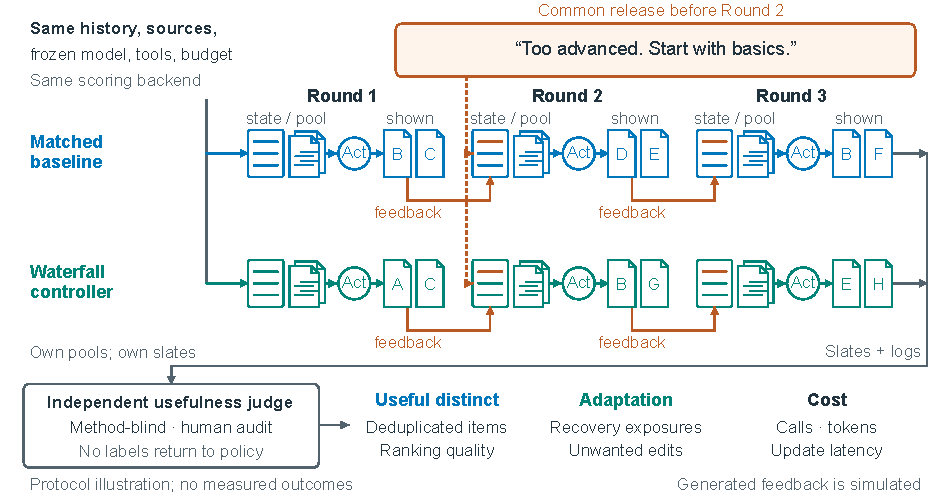
\includegraphics[width=\textwidth]{figures/waterfall-evaluation.pdf}
\caption{Proposed multi-round evaluation under matched starting conditions. Each method produces its own displayed slate (letters are illustrative item identifiers) and receives feedback only on that slate. Feedback updates its next state. A separate, method-blind judge assesses usefulness, with a human audit; adaptation and cost are measured from trajectory logs. Judge labels do not return to either policy. Three rounds illustrate the protocol, not observed outcomes or the final horizon.}
\label{fig:evaluation}
\end{figure*}


\subsection{Data and Environments}

\paragraph{A shared benchmark starting point.}
ClawRec-SimBench \citep{wu2026clawrec} supplies user scenarios and history-based recommendation tasks. We propose reproducing its single-step setting before extending the interaction horizon. All methods receive the same permitted history, sources, tool interface, and budget. They may retrieve different candidates: forcing a common candidate set in this experiment would remove the acquisition decision being tested.

\paragraph{A multi-round extension.}
The primary proposed experiment uses versioned snapshots of real content from multiple sources and replayable retrieval interfaces. Scenario annotations specify an initial goal and later changes, such as a new task, a difficulty correction, or a request to avoid repeated content. The controller sees only the instructions and behaviors released at the relevant step, not the hidden scenario description.

Each method receives feedback conditional on the items it actually displays. If those reactions are generated by a simulator, they are explicitly synthetic. We will separate the feedback generator from the usefulness judge, audit both with human judgments, and test sensitivity to different feedback generators. The same scenario and random seeds support paired comparisons, but do not require different policies to receive identical item-level reactions.

The extension needs user-disjoint development and test sets, with scenario-template overlap also controlled. Dataset size, interaction horizon, source snapshots, and simulator configuration remain to be fixed before test evaluation. A separate live-source run can assess retrieval failures and latency; snapshot experiments alone cannot establish performance on a changing web.

\paragraph{Recorded behavior.}
KuaiRand-1K provides a complementary temporal evaluation \citep{gao2022kuairand}. At each evaluation point, the model can use only earlier observations to predict or rank later recorded feedback. We retain native event meanings and report which content-side metadata are available. Aggregate item features calculated using future observations are excluded. Playback signals are not treated as equivalent to Waterfall's visible-card duration.

This experiment tests whether state updates help on real behavior under the recorded exposure policy. It does not show how those users would respond to an alternative Waterfall feed. Unobserved items are not automatically negative examples. Random-exposure subsets can support narrower analyses when their sampling assumptions apply.

\paragraph{Text and human validation.}
A controlled candidate-ranking experiment can use MIND's textual news and impression labels \citep{wu2020mind}, or instruction-oriented tasks from iAgent's evaluation \citep{xu-etal-2025-iagent}. The choice should follow the final language claim rather than add unrelated benchmark scores. A subsequent user study should compare the full method with the strongest matched baseline, counterbalance condition order, and ask users to judge usefulness and goal satisfaction directly. Its sample size and analysis require a pilot and an approved study protocol.

\subsection{Matched Baselines}

The main comparisons use the same frozen language model, available history, source access, scoring backend, and resource caps wherever the method permits. Adaptations to published systems are reported explicitly.

\begin{enumerate}
    \item \textbf{Fixed pipeline:} update stage-specific state views, acquire, and rank in a predetermined order with fixed triggers.
    \item \textbf{Shared-state pipeline:} expose the same scoped state to every stage but retain the fixed schedule.
    \item \textbf{General agent:} a ReAct-style policy with the same observations and four action types.
    \item \textbf{ClawRec:} the closest complete system, evaluated in the same environment with documented adapters.
    \item \textbf{Waterfall prototype:} the existing bounded-edit implementation.
    \item \textbf{Waterfall controller:} the proposed candidate-aware policy with scoped updates.
\end{enumerate}

RecBot and MARS motivate additional command-planning and memory substitutions when their interfaces can be adapted fairly. Their published scores must not be compared directly with scores from a different environment. We will report both matched-component comparisons and any reproduction that requires a different model or backend, keeping their interpretations separate.

\subsection{Metrics}

\paragraph{Usefulness over time.}
The primary outcome is the number of useful, distinct items encountered across a trajectory, as in Equation~\ref{eq:objective}. We also report the proportion of useful items in each top-$k$ slate, duplicate exposure, and explicit constraint violations. A short slate is reported as such; missing positions contribute zero to useful-items@$k$, preventing a method from improving precision by returning almost nothing. Clicks and dwell time are feedback features, not direct definitions of satisfaction.

\paragraph{Retrieval and ranking.}
In a fixed corpus with known relevant items, Recall@$k$ is the fraction retrieved. If ten relevant items exist and seven are returned, recall is $0.7$. With incomplete judgments, we report coverage of a pooled, assessed set and identify that limit.

Ranking is evaluated with nDCG@$k$ \citep{jarvelin2002cumulated}, which gives more credit when useful items appear earlier. For acquisition-inclusive comparisons, the ideal ordering comes from a common judged pool formed across methods and a shared retrieval baseline. It is not recomputed from each method's own returned list. For ranking-only comparisons, every method receives the same candidates. Absolute usefulness is reported with nDCG because pooled judgments remain incomplete.

\paragraph{Adaptation and state errors.}
After an explicit goal change, we measure the number of exposures until recommendations meet a prespecified usefulness threshold for a prespecified consecutive window. Thresholds are set on development data. Trajectories that never recover remain failures rather than disappearing from the mean. We also measure changes to unrelated persistent preferences, retention of explicit corrections, and repeated recommendations after a novelty complaint.

\paragraph{Resources and reliability.}
We report source calls, input and output tokens, time to the first updated useful slate, median and 95th-percentile update latency, invalid action rates, and source failures. Quality is compared at several common budgets. No single weighted score should hide a gain purchased through substantially more retrieval or model computation.

\subsection{Ablations and Analysis}

The first ablation freezes memory updates while retaining retrieval and ranking. The second fixes queries while allowing other state to change. The third fixes the ranking context while retaining acquisition and memory updates. A fourth preserves the full state and action set but replaces candidate-aware control with a fixed schedule. These variants retain functioning stages instead of deleting entire capabilities.

A factorial comparison of memory adaptation and query adaptation can test their interaction. If $J_{ij}$ denotes trajectory usefulness with the two adaptations enabled or disabled, the contrast
\begin{equation}
\Delta=J_{11}-J_{10}-J_{01}+J_{00}
\end{equation}
measures non-additivity at a common budget. A positive contrast would support complementarity in that setting; it would not establish a general theorem about unified agents. Matched-cost retry and exploration controls are needed to separate coordination from extra opportunities to find content.

Usefulness judgments are collected without revealing the producing method. Large-scale model judgments require independent human checks and an agreement report. Uncertainty is estimated by resampling users or complete trajectories, not individual clicks from the same user. Error analysis should distinguish incorrect feedback interpretation, inappropriate persistence, candidate shortages, ranking mistakes, and tool failures.

\section{Empirical Status}
\label{sec:status}

No experiment in Section~\ref{sec:evaluation} has been run for this draft. We therefore report no performance table, significance claim, user-study outcome, or ablation result. The completed study must establish whether the proposed controller improves on the shared-state pipeline, general agent, and ClawRec at comparable cost. Gains over a static profile alone would not support the central coordination claim.

\section{Conclusion}

Waterfall frames continual search and recommendation as a decision about what to acquire, what to show, and what to change in user state. The proposed controller connects these operations through scoped feedback interpretation and an explicit check of the available candidates. The existing prototype provides bounded memory and query edits; the wider controller and its evaluation are still pending. The planned comparisons are designed to determine whether coordination adds value beyond shared context and access to the same tools.

\section*{Limitations}

This manuscript is an initial method and evaluation draft, not a completed empirical study. The broader controller has not been implemented or validated, and source inspection of the existing prototype does not establish runtime correctness or recommendation quality. Concrete model versions, prompts, budgets, dataset splits, and study sizes remain to be fixed and reported.

The proposed controller depends on imperfect interpretations of both language and behavior. Candidate sufficiency is estimated by a scorer; a miscalibrated score can stop acquisition too early or cause wasteful searching. Task boundaries may be unclear, and repeated behavior does not necessarily identify a stable preference. These assumptions require direct ablations.

Synthetic users may reward the reasoning style or preferences of the model that generated them. Real logs reduce that concern but contain exposure bias and do not reveal counterfactual responses to arbitrary recommendations. Content snapshots improve repeatability while omitting changes in availability and source behavior. A small human study would provide limited evidence about broader populations.

Our literature comparison identifies close precedents rather than proving the absence of equivalent systems. In particular, full-workflow agents, editable memory, and retrieval--ranking coupling already exist. Any eventual novelty claim must be stated at the level of the implemented mechanism and supported by matched experiments.

\section*{Ethical Considerations}

Persistent behavioral memory can reveal sensitive interests even when raw events appear innocuous. The proposed data flow should use only authorized sources, minimize retained personal information, and allow users to inspect, correct, and delete learned state. Retrieval permissions must remain separate from inferred preferences. Personal histories should not be sent to an external model provider without an appropriate consent and data-handling basis.

Public datasets and source content remain subject to their licenses and access conditions. A released benchmark should document provenance and redistribute only permitted material. Identifiers, access tokens, and private user content must not appear in prompts, logs, or released examples.

No new participants were recruited for this draft. A future study requires the applicable institutional ethics review, informed consent, a withdrawal mechanism, and a stated retention policy. Engagement should not be optimized as a substitute for user benefit: the proposed evaluation includes explicit usefulness, goal satisfaction, and unwanted preference changes.

% Review manuscripts must not contain an Acknowledgments section.
% AI-assistance disclosure and unresolved author decisions are in DRAFT_NOTES.md.

\bibliography{waterfall}

\appendix

\section{Event Semantics and Dataset Mapping}
\label{app:events}

Table~\ref{tab:events} defines a mapping for the proposed experiments. It preserves differences between measurements instead of forcing every source into an interchangeable reward. Missing fields remain missing. The Waterfall entries describe available prototype signals; dataset entries describe the corresponding public fields.

\begin{table*}[t]
\centering
\begin{tabular}{>{\raggedright\arraybackslash}p{0.16\textwidth}>{\raggedright\arraybackslash}p{0.21\textwidth}>{\raggedright\arraybackslash}p{0.21\textwidth}>{\raggedright\arraybackslash}p{0.29\textwidth}}
\toprule
Observation & Waterfall & Public-data counterpart & Interpretation boundary \\
\midrule
Explicit positive reaction & Like event & KuaiRand \texttt{is\_like} & Supports the displayed item; does not alone establish a permanent broad interest. \\
Explicit negative reaction & Dislike event & KuaiRand \texttt{is\_hate} & Distinguish a negative reaction from removal of a previous like. \\
Opening content & Open event with available duration & MIND impression click; KuaiRand \texttt{is\_click} & KuaiRand's click field depends on interface context and can encode valid play. \\
Time spent & Card visibility or supported open-duration signal & KuaiRand \texttt{play\_time\_ms} & Visibility and playback measure different behavior; thresholds are not transferred unchanged. \\
Language correction & User utterance & Scenario annotations or instruction-oriented tasks & Preserve wording and time of availability; generated corrections must be marked synthetic. \\
No observed reaction & Exposure without an explicit reaction & Logged exposure with available feedback & Absence of a like is not a dislike; an unexposed item is not a negative example. \\
\bottomrule
\end{tabular}
\caption{Proposed event mapping. Dataset semantics follow their official descriptions \citep{gao2022kuairand,wu2020mind}. This is not a claim that public logs contain all Waterfall events or language instructions.}
\label{tab:events}
\end{table*}

The current behavioral agent accepts a JSON object with memory edits and a search-term update. Memory edits strengthen or weaken entries. A null search-term field retains the current set, an empty list clears it, and a nonempty list replaces it. The proposed scoped-state extension would add explicit evidence references and scope; those fields should not be described as already present in the prototype.

\section{Illustrative Decision Trace}
\label{app:trace}

The following example is constructed to explain the proposed policy; it is not an observed experiment.

\paragraph{Initial request.}
The user asks for help learning night photography after buying a camera. The system records a current learning task and searches for relevant lessons. It does not infer that the user wants to buy another camera.

\paragraph{Difficulty correction.}
The user says, ``These are too advanced. Start with the basics.'' The interpreter proposes a task-scoped difficulty correction. If the pool already contains enough beginner lessons, the executor reranks it without another search. If it does not, acquisition uses the revised learning requirement.

\paragraph{Novelty correction.}
The user says, ``I have already read these.'' The system excludes the corresponding duplicate groups from subsequent exposure. This observation does not weaken the photography preference by itself. It may require acquisition if too few unseen lessons remain.

\paragraph{Temporary task.}
The user requests a weekend travel itinerary. This requirement governs the active task. Ending it removes its task-specific influence without deleting the earlier photography evidence. Whether the proposed scope handling achieves this behavior reliably is an empirical question.

\section{Reproducibility Record to Complete}
\label{app:reproducibility}

Before evaluation, the study must record model and provider versions, complete prompts, decoding settings, the action schema, source adapters, snapshot dates, and budget enforcement. It must also fix the candidate eligibility threshold, update and exploration rules, maximum acquisition attempts, horizon, user splits, scenario construction, and feedback generators.

The released evaluation specification should include annotation instructions, duplicate grouping, the common relevance pool, metric implementations, failure handling, and user-level uncertainty estimates. Baseline adaptations and departures from authors' reference implementations need explicit documentation. These items are requirements of the proposed study, not artifacts already released.

\end{document}
